% arara: xelatex
% arara: xelatex
% arara: xelatex

% options:
% thesis=B bachelor's thesis
% thesis=M master's thesis
% czech thesis in Czech language
% english thesis in English language
% hidelinks remove colour boxes around hyperlinks

\documentclass[thesis=M,english]{FITthesis}[2012/10/20]

\usepackage[utf8]{inputenc}

\usepackage{graphicx} %graphics files inclusion
% \usepackage{subfig} %subfigures
% \usepackage{amsmath} %advanced maths
% \usepackage{amssymb} %additional math symbols

\usepackage{dirtree} %directory tree visualisation

% ADDED BY ME
\usepackage{blindtext} % lorem ipsum
\usepackage{todonotes} 

\newcommand{\todotext}[1]{\textcolor{red}{\textbf{[[#1]]}}}
\definecolor{mygray}{gray}{0.6}
\newcommand{\blind}[1][1]{\textcolor{mygray}{\Blindtext[#1][1]}}

\setlength{\fboxsep}{0.005pt}
\newcommand{\tmpframe}[1]{\fbox{#1}}
%\renewcommand{\tmpframe}[1]{#1}

\let\myCite\cite
\renewcommand\cite{\unskip~\myCite}
\let\myRef\ref
\renewcommand\ref{\unskip~\myRef}

\newcommand\hatx{\^{}}


% list of acronyms
%\usepackage[acronym,nonumberlist,toc,numberedsection=autolabel,nomain]{glossaries}
\iflanguage{czech}{\renewcommand*{\acronymname}{Seznam pou{\v z}it{\' y}ch zkratek}}{}
%\makeglossaries

\newcommand{\tg}{\mathop{\mathrm{tg}}} %cesky tangens
\newcommand{\cotg}{\mathop{\mathrm{cotg}}} %cesky cotangens

% % % % % % % % % % % % % % % % % % % % % % % % % % % % % % % % % % % 
% % % % % % % % % % % % % % % % % % % % % % % % % % % % % % % % % % % 
\department{Department of theoretical computer science}
\title{Contextual Shell History}
\authorGN{Šimon} %author's given name/names
\authorFN{Let} %author's surname
\authorWithDegrees{Bc. Šimon Let} %author's name with academic degrees
\author{Šimon Let} %author's name without academic degrees
\supervisor{Ing. Lukáš Bařinka}
% my BP thesis: I~would like to thank my supervisor Ing. V{\' i}t List{\' i}k, without his assistance and guidance this thesis would have not be accomplished.
% \par Then I~would like to thank Ing. Michal Bukovsk{\' y} along with his whole Email.cz team in Seznam.cz for letting me work with them and use their data.
% \par My thanks also goes to RNDr. Jana Strakov{\' a} at. el for developing Nametag, Named entity recognition solution, I~used in this thesis, and answering my questions.
% \par Finally I~want to thank my family and friends for their support trough my whole studies.
\acknowledgements{TODO: I would like to thank my supervisor Ing. Lukáš Bařinka for his guidance, my colleagues and friends for their feedback, hundreds of people who downloaded this project for their trust, and my family for support during writing this thesis. Installfest for accepting my talk about this project. Github users who submitted issues and pull requests to the project.}
\abstractCS{\todotext{TODO: CZ abstrakt}  \blind[2]}
\abstractEN{\todotext{TODO: abstract} This thesis is an enhancement for standard shell history. It records shell history with context. It uses the recorded context to make it easier to find relevant history records and to make it possible to search search history using context explicitly.

\blind[2]
}
\placeForDeclarationOfAuthenticity{Prague} %where you have signed the declaration
\keywordsCS{Shell, Příkazová řádka, Historie shellu, Nástroje produktivity}
\keywordsEN{Shell, Command line, Shell history, Productivity tools}
\declarationOfAuthenticityOption{1} %select as appropriate, according to the desired license
% \website{https://github.com/curusarn/master-thesis} %optional URL (remove entirely if you have no URL for this thesis) TODO: put the thesis up

\begin{document}

%\newacronym{GUI}{GUI}{Graphical User Interface}
%\newacronym{CLI}{CLI}{Command Line Interface}
%\newacronym{GNU}{GNU}{GNU's Not Unix!}
\begin{introduction}



Classic command line interfaces were mostly replaced by GUIs in consumer software \cite{norman2007ui}. \todo{REF?} However, many professionals around the world still rely on UNIX shells to achieve their daily tasks. CLIs are generally not replaceable by GUIs because GUIs do not scale well when the number of available actions is high \cite{norman2007ui}. 

More than half of all developers use Unix-based operating systems\footnote{According to \cite{stackoverflow2019devsurvey}, 25.6\% and 26.8\% of developers uses Linux and MacOS respectively.}. 
About half of all developers have been working with Linux during year 2018. \cite{stackoverflow2019devsurvey} 

Default shell on GNU/Linux is bash \cite{ramey1994gnubash} and default shell on MacOS is zsh since October 2019 \cite{apple2019zsh}. In this work we primarily focus on these two popular shells.
\todo{TODO: polish the argument why is this work relevant \hatx\hatx\hatx}

The standard shell history contains records with basic information about previously executed command lines. Each record only contains following details: the command line, timedate of the execution, and the duration of the execution\footnote{Duration is only available in zsh and only when it is enabled.\cite{zshdocs}}. 

Additionally, it is quite common to use shell configuration\footnote{\todotext{e.g. bash: histocontrol=ignoredups\cite{bashman}; zsh: HIST\_SAVE\_NO\_DUPS\cite{zshdocs}}} to prune duplicates from the history. This removes more information from history because the original command line sequences are lost.

As we can see the standard shell history contains only very basic information about executed command lines.
There is much more contextual data available at the time of command line execution e.g. present working directory, exit status, and previously executed commands. In this work, we explore the possibilities of using the contextual data about executed commands to increase the usefulness of shell history.



% BAD: This limits the potential of standard shell history utilities because shell usage is contextual. is not generally used to run ad-hoc commands but 

% MORE PRACTICAL: When using shells you likely do not run individual commands completely independently of each other. But instead run commands as parts of different workflows that 

\todotext{TODO: describe the contents of this work / layout} We start by analysing shell history features to understand advantages and disadvantages of standard shell history. We research existing history tools to see what ideas were already explored, which features work and which do not. 

After that, we focus on people. We start broad and research how people use computer tools in general. Then we move on to examining how people use shell and shell history.

Next, we focus on the contextual information; We cover what information is available to be saved at the time of command line execution and we discuss how it could be used to enhance shell history.

At this point we move on to design(ing) ...
\todotext{TODO: finish this intro}


\blind[2]

\end{introduction}


\chapter{Analysis}

\todotext{TODO: describe layout/contents of the chapter}

\blind

\section{Shells, existing shell history features and tools}


\todotext{TODO: describe contents of this section}

\blind

\subsection{Recurrent systems}

\todotext{TODO: explain what are recurrent systems}

\blind

\subsection{Shells and built-in history features}

\todo{TODO: shell history configurations options - here or in a separate section}

\blind[4]

\todotext{TODO: short conclusion about shells}

\subsection{History features of Read-eval-print loops}

\blind[1]

\subsection{Existing history tools \todotext{TODO: split into more subsections}}

\blind[4]

\todotext{TODO: short conclusion about history tools}

\section{How people use shell and shell history}

\todotext{TODO: intro - why we analyze people}

\blind

\todotext{TODO: introduce personas}

\todotext{TODO: describe use cases}

\blind[2]

\subsection{How people use tools}

Dummy citation \cite{greenberg1993computer}

\blind[2]

\subsection{How people use shell}

\todotext{TODO: Greenberg conducted a study in his work \cite{greenberg1993computer} in 19XX which provides a lot of insight into how people use shell. It's not obvious that conclusions and ideas in the work still hold. To make sure that the usage of shell didn't change to the point where we can't use the ideas anymore. }

plots:

Figure 3.1. The normalized command frequency, compared with Zipf.

\begin{figure}
  \tmpframe{\includegraphics[width=\linewidth]{figures/greenberg/plot_ref_zipf-cmd-frq.png}}
  \caption{The normalized command frequency, compared with Zipf. (Greenberg)}
\end{figure}

\begin{figure}
  \tmpframe{\includegraphics[width=\linewidth]{figures/greenberg_new/plot_zipf-cmd-frq.png}}
  \caption{The normalized command frequency, compared with Zipf.}
\end{figure}


Figure 3.2. Command vocabulary size vs. the number of command
lines entered for four individuals.

\begin{figure}
  \tmpframe{\includegraphics[width=\linewidth]{figures/greenberg/plot_ref_cmd-vocab-size.png}}
  \caption{Command vocabulary size vs. the number of command
lines entered for four individuals. (Greenberg)}
\end{figure}

\begin{figure}
  \tmpframe{\includegraphics[width=\linewidth]{figures/greenberg_new/plot_cmd-vocab-size.png}}
  \caption{Command vocabulary size vs. the number of command
lines entered for \todotext{N individuals}}
\end{figure}


Figure 3.3. Sequential structure of UNIX command usage, from Figure 4
in Hanson et al. (1984).

\begin{figure}
  \tmpframe{\includegraphics[width=\linewidth]{figures/greenberg/graph_ref_cmd-sequences.png}}
  \caption{Sequential structure of UNIX command usage, from Figure 4
in Hanson et al. (1984). (Greenberg)}
\end{figure}

\begin{figure}
  \tmpframe{\includegraphics[width=\linewidth]{figures/greenberg_new/graph_cmd-sequences.pdf}}
  \caption{Sequential structure of command usage.}
\end{figure}


Table 5.2. The average recurrence rate of the four sample UNIX user
groups

\begin{figure}
  \tmpframe{\includegraphics[width=\linewidth]{figures/greenberg/table_recurr-rate-in-different-samples.png}}
  \caption{The average recurrence rate of the four sample UNIX user
groups (Greenberg)}
\end{figure}

Figure 5.6. Command line vocabulary size vs. the number of commands
entered for four typical individuals.

\begin{figure}
  \tmpframe{\includegraphics[width=\linewidth]{figures/greenberg/plot_ref_cmdline-vocab-size.png}}
  \caption{Command line vocabulary size vs. the number of commands
entered for four typical individuals. (Greenberg)}
\end{figure}

\begin{figure}
  \tmpframe{\includegraphics[width=\linewidth]{figures/greenberg_new/plot_cmdline-vocab-size.png}}
  \caption{Command line vocabulary size vs. the number of commands
entered for a single experienced programmer \todotext{TODO: title}}
\end{figure}


\blind[4]

\subsection{How people use shell history}

\blind[4]


\todotext{TODO: conclusion of the chapter}

\blind

\section{Available contextual information}

\todotext{TODO: intro}

\subsection{Directly available contextual information}

\blind[2]

\subsection{Derivable contextual information}

\blind[2]

\todotext{TODO: conclusion of the section}



\chapter{Design}
\todotext{TODO: intro describe contents of the chapter}

\blind
\todo{order of design chapters can change}
\section{Recording contextual history}

\todotext{TODO: what to record}

\blind[2]

\section{Front-end and User interaction}\todo{I don't like the title}

\todotext{TODO: intro}

\blind

\subsection{Standard history features}

\todotext{TODO: describe why it's important to respect the standard history features}

\todotext{TODO: which history features are we keeping/enhancing/leaving intact}

\blind[3]

\todotext{TODO: conclusion for further design ?}



\subsection{Core ideas, principals, design decisions, and features}\todo{weird title}

\todotext{TODO: intro: ideas in this chapter are essential for this work / project}

\todotext{TODO: features of the project - weird todo}

\blind[3]

\subsection{Possible features}

\todotext{TODO: intro: this section describes features that were considered during the design - for each feature we evaluate how well it would fit with the rest of the design. Some of the features were explicitly suggested by users and some features are included for the sake of completeness (because they make sense).}

\todo{TODO: list the features}


\section{Back-end}\todo{I don't like the title}

\blind

\section{Testing the design}

\todotext{TODO: explain why we want to test the design - intro}

\todotext{TODO: principals, guidelines, etc. are we are using}

\blind[3]

\chapter{Implementation}
\todotext{describe layout/contents of the chapter}

\blind

\section{Daemon}\todo{do we need this or is introduction enough}

\blind

\section{Choosing Go}

\blind[3]

\section{Recording shell history with context}

\blind

\subsection{History format}

\todotext{NOTE: both on disk and in transfer}

\blind

\subsection{Shell integration and hooks}

\blind

\subsection{History record merging}

\blind

\section{Custom arrow key bindings}

\todotext{TODO: intro: we want arrow key bindings to be able to record usage related metadata + it's a good idea to have the option to customize and use context to enhance arrow key bindings. Plus impossibility of gathering usage data and using the default bindings (at least in bash)}

\blind

\subsection{Keybinding custom functions in zsh}

\blind

\subsection{Keybinding custom functions in bash}

\blind

\subsection{Reverting keybindings}

\blind

\subsection{Universal keybinding library}
\todotext{TODO: explain why: as you see bash and zsh have a different ways of supporting custom keybindings. To simplify our codebase we extracted the keybind setting logic into a library. (unified way to set keybindings)}

\blind

\subsection{Performance issues of custom keybindings in bash}

\blind


\section{Fullscreen command line history searching application}

\todo{TODO: subsections}


\section{Daemon components}

\todotext{TODO: describe why we need components}

\begin{figure}
  \tmpframe{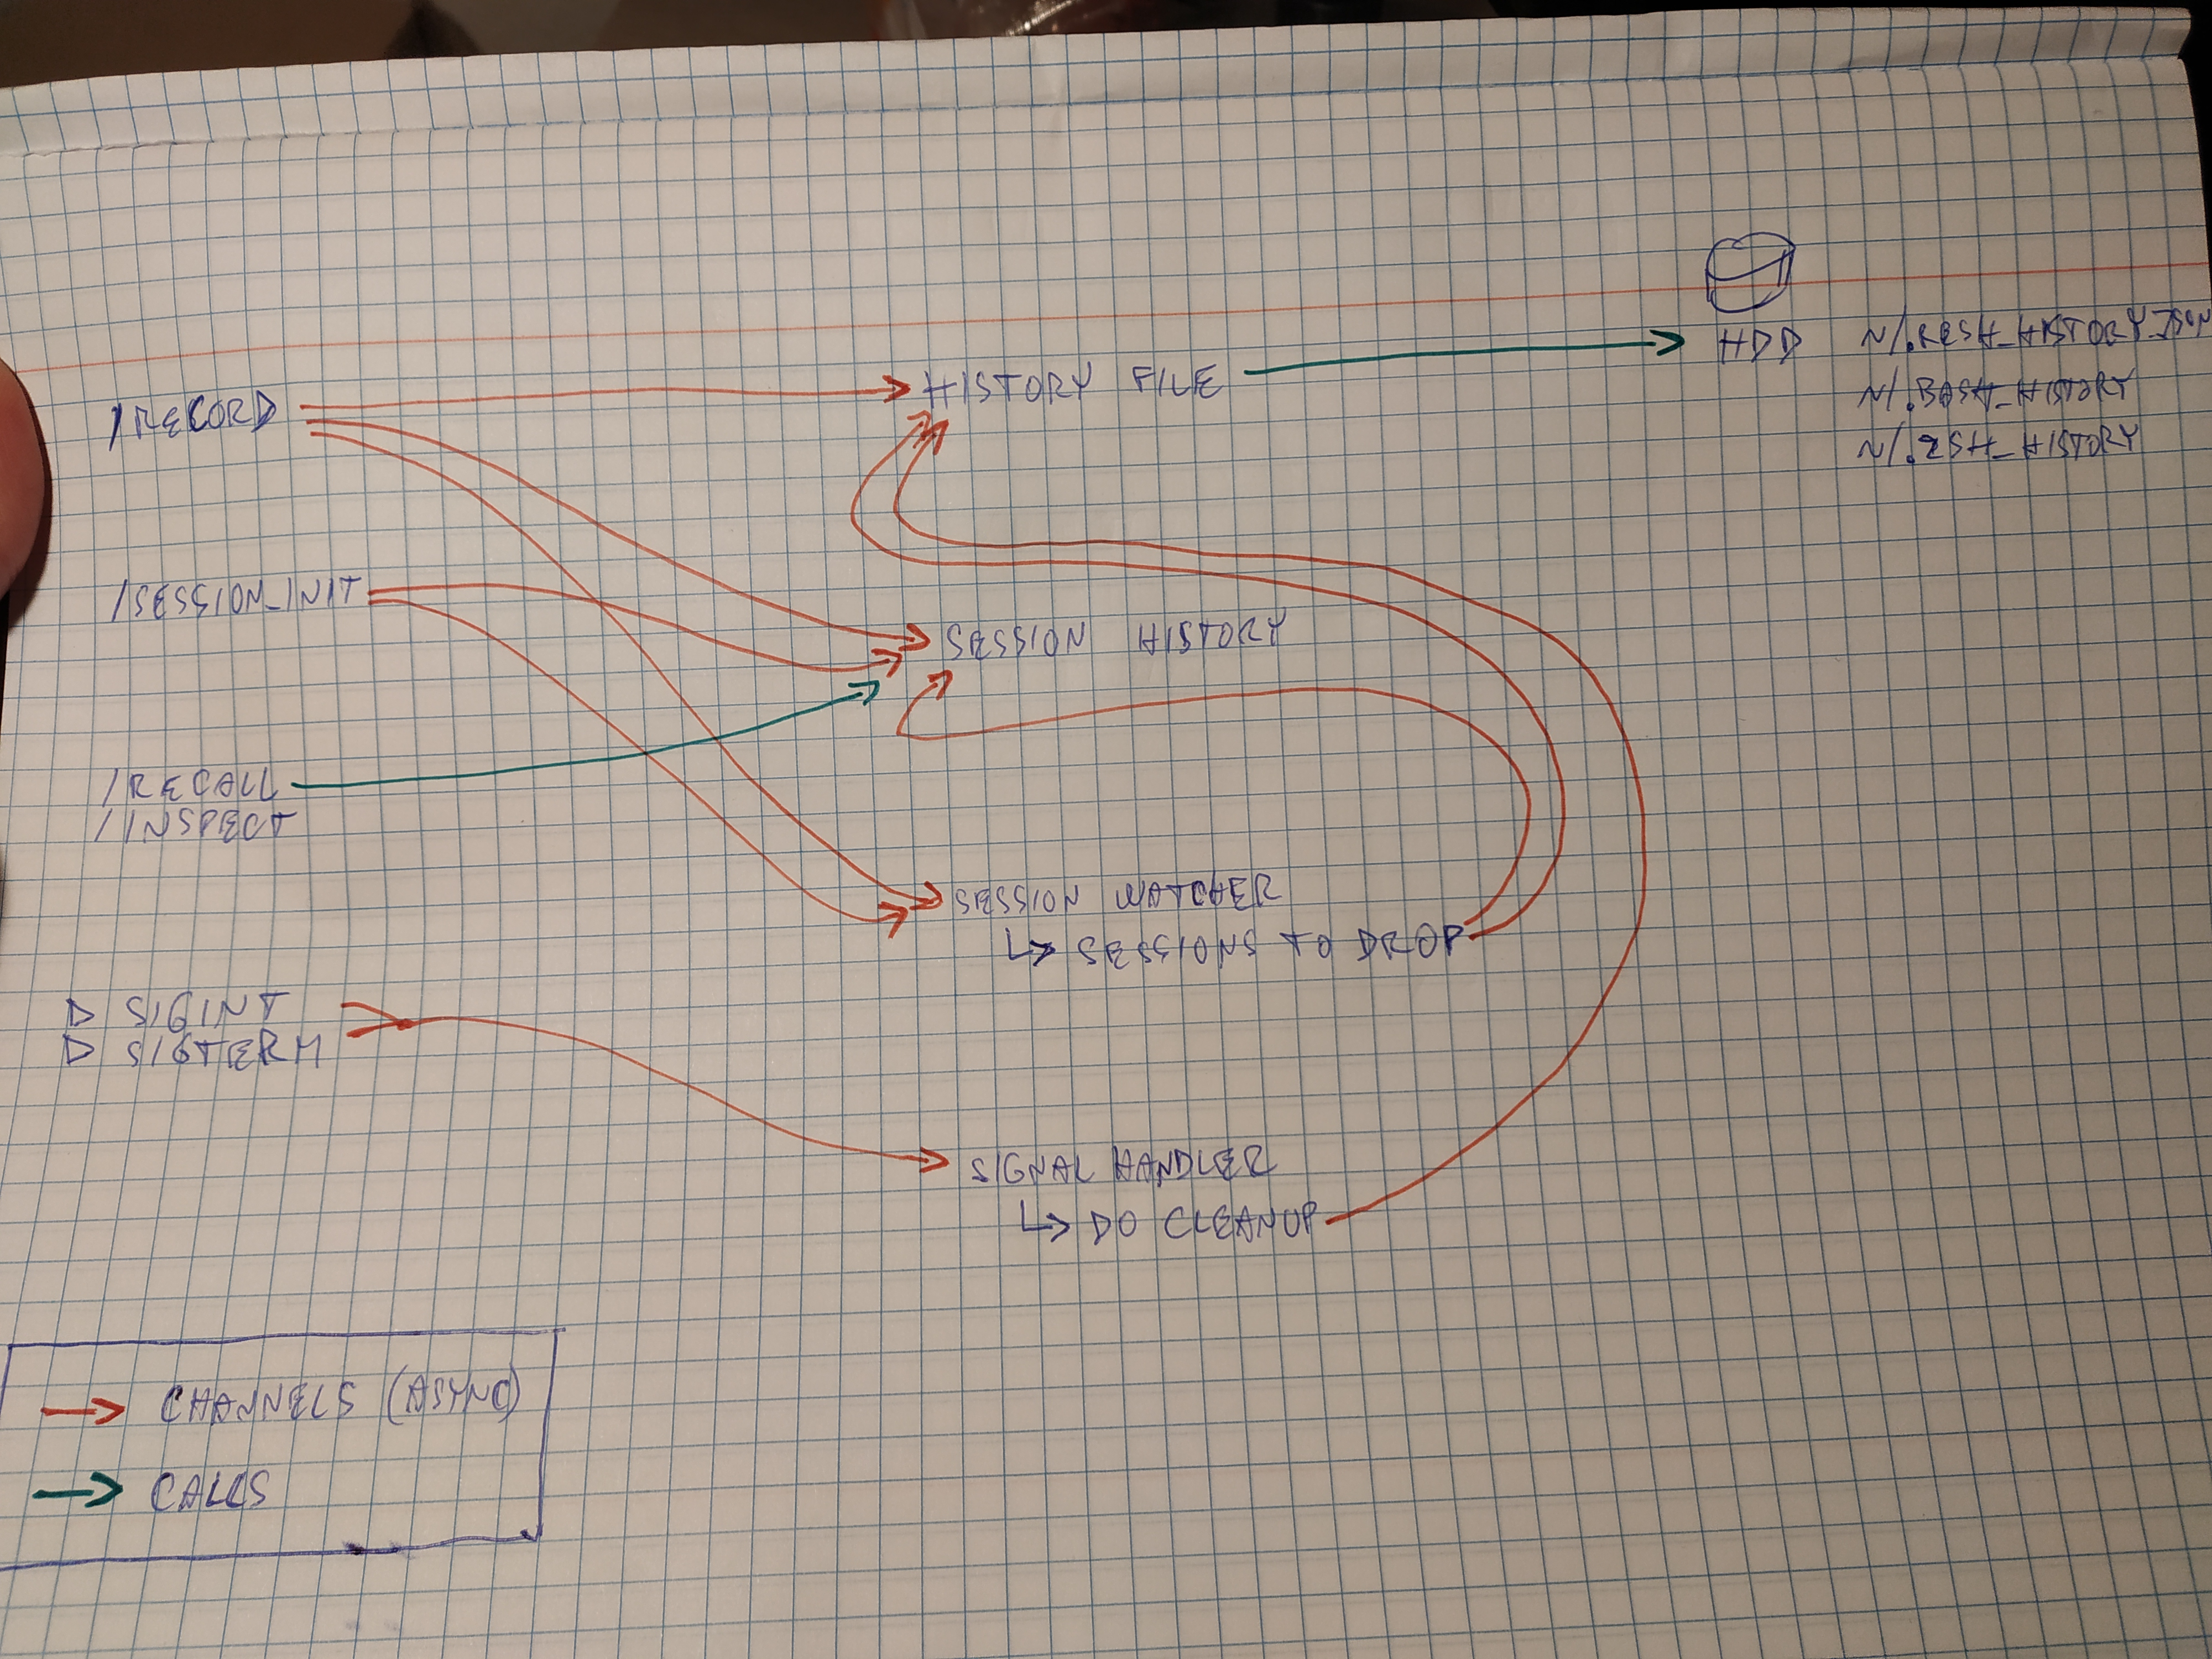
\includegraphics[width=\linewidth]{figures/daemon-components.jpg}}
  \caption{One image. \todotext{TODO: write a title}}
  \label{fig:TODO}
\end{figure}

\subsection{Server}

\subsection{History file}

\subsection{Session history}
\todotext{TODO: explain: there are implications for the daemon if we want responsive arrow key bindings}

\subsection{Expired session tracking}


\subsection{Signal handling}

\blind

\section{Control and configuration}

\blind

\section{Installation, updates, and build process}

\todotext{TODO: explain how simple the installation is. plus updates.}

\blind

\subsection{Installation and updates}
\todotext{TODO: explain how installation works}

\blind

\subsection{Production and development build process}
\todotext{TODO: explain the build process}

\blind[2]


\chapter{Testing and Evaluation}

\todotext{TODO: describe layout/contents of the chapter}

\todotext{TODO: describe how history tools can be usable}

\todotext{TODO: describe what influences usability of the tools}

\todotext{TODO: explain which parts of the system should be tested and why}

\blind[3]

\section{Metrics}

\todotext{TODO: describe why we use metrics}

\subsection{Metrics traditionally used to evaluate history tools}\todo{break down into more subsections ?}

\todotext{TODO: describe which metrics were used for history tools in the past}

\subsection{Newly suggested metrics}\todo{break down into more subsections ?}

\todotext{TODO: suggest new metrics + explain how they are better than the original ones}

\subsection{Evaluation using suggested metrics}

\todotext{TODO: explain used methods}

\todotext{TODO: use metrics to evaluate usefulness of the work}


\section{Use cases}



\begin{conclusion}

\todotext{TODO: rewrite conclusion}

I have analysed shell history features available in current shells. I explored available history tools and found both positive and negative inspiration.

\par I have found previous research on how people use shell and shell history.  
I have collected a sample of shell history. I have analyzed the collected usage data and compared it to data used in existing research. I have found which characteristics of shell usage changed over time and which characteristics stayed the same. I have concluded that most of the principals and ideas from the existing research do still hold. I have found out that potential recalled characters increased 4 times since the study was conducted. This and other differences reinforced the idea that it makes sense to design and develop new history related tools. 

\par I have conducted a market research to find out how people interact with shell history and what are the workflows that are not well supported nowadays. I have modelled personas representing target users of the system. I have put together use cases based on actual shell history I have collected.
I have designed a contextual shell history tools based on problems and suggestions from existing literature, user-centered design guidelines and principals, information learned via market research, and modelled personas.
I have actively sought feedback from users during both design and implementation. 

I have used usability principals and heuristics to test and evaluate the design.

\par I have implemented a significant portion of the design. The project unobtrusively records shell history with context. It does both use context to offer relevant history records and for searching via fullscreen command line application.
I have made sure that it's easy to install, update, configure and use. I have shared the resulting implementation with community and received overwhelmingly positive feedback and interest of contributors. Project was downloaded and installed over 5 hundred times since January. Github page of the project consistently attracts daily visitors.  

\par I have described a number of possible metrics. I have explained why simple metrics are not sufficient. I have described the drawbacks of metrics in general. I have suggested meaningful metrics that can be used to evaluate shell history tools. I have used the suggested metrics to evaluate my implementation where possible. 

\par I have used modelled personas and use cases to evaluate utility and usability of the system.
I have used real life user data to evaluate user experience of the solution.


I have made it easier to collect and study usage of shell and shell history in future research.
I have proved that having contextual shell history brings many benefits. 
I have demonstrated public demand for history tools. 
I have created a universal shell library for binding custom functions to keys with the option to revert to previous state. 




\todotext{TODO: write future work}

\end{conclusion}

\bibliographystyle{iso690.bst}
\bibliography{ref}

\appendix

%\printglossaries

\chapter{Contents of SD card}\label{app:SDcontent}

\todotext{TODO: Visualise the contents of enclosed media. Use of dirtree is recommended. Note that directories src and text with appropriate contents are mandatory.}


\begin{figure}
	\dirtree{%
		.1 readme.txt\DTcomment{the file with CD contents description}.
		.1 data\DTcomment{the data files directory}.
		.2 graphs\DTcomment{the directory of graphs of experiments}.
		.3 *.eps\DTcomment{the B/W graphs}.
		.3 *.png\DTcomment{the color graphs}.
		.3 *.dat\DTcomment{the graphs data files}.
		.1 exe\DTcomment{the directory with executable WBDCM program}.
		.2 wbdcm\DTcomment{the WBDCM program executable (UNIX)}.
		.2 wbdcm.exe\DTcomment{the WBDCM program executable (Windows)}.
		.1 src\DTcomment{the directory of source codes}.
		.2 wbdcm\DTcomment{the directory of WBDCM program}.
		.3 Makefile\DTcomment{the makefile of WBDCM program (UNIX)}.
		.2 thesis\DTcomment{the directory of \LaTeX{} source codes of the thesis}.
		.3 figures\DTcomment{the thesis figures directory}.
		.3 *.tex\DTcomment{the \LaTeX{} source code files of the thesis}.
		.1 text\DTcomment{the thesis text directory}.
		.2 thesis.pdf\DTcomment{the Diploma thesis in PDF format}.
		.2 thesis.ps\DTcomment{the Diploma thesis in PS format}.
	}
\end{figure}


\end{document}
